% generated from JIRA project LVV
% using template at /usr/share/miniconda/envs/docsteady-env/lib/python3.7/site-packages/docsteady/templates/tpr.latex.jinja2.
% using docsteady version 2.2.9
% Please do not edit -- update information in Jira instead
\documentclass[DM,lsstdraft,STR,toc]{lsstdoc}
\usepackage{geometry}
\usepackage{longtable,booktabs}
\usepackage{enumitem}
\usepackage{arydshln}
\usepackage{attachfile}
\usepackage{array}
\usepackage{dashrule}

\newcolumntype{L}[1]{>{\raggedright\let\newline\\\arraybackslash\hspace{0pt}}p{#1}}

\input meta.tex

\newcommand{\attachmentsUrl}{https://github.com/\gitorg/\lsstDocType-\lsstDocNum/blob/\gitref/attachments}
\providecommand{\tightlist}{
  \setlength{\itemsep}{0pt}\setlength{\parskip}{0pt}}

\setcounter{tocdepth}{4}

\begin{document}

\def\milestoneName{RSP on the Interim Data Facility (IDF) is ready for DP0.2}
\def\milestoneId{LDM-503-RSPa}
\def\product{LSP Services}

\setDocCompact{true}

\title{LDM-503-RSPa: RSP on the Interim Data Facility (IDF) is ready for DP0.2 Test Plan and Report}
\setDocRef{\lsstDocType-\lsstDocNum}
\date{ 2022-09-16 }
\author{ Gregory Dubois-Felsmann }

% Most recent last
\setDocChangeRecord{
\addtohist{1.0}{2022-09-16}{Initial complete version of test plan}{Gregory Dubois-Felsmann}
}

\setDocCurator{Gregory Dubois-Felsmann}
\setDocUpstreamLocation{\url{https://github.com/lsst-dm/\lsstDocType-\lsstDocNum}}
\setDocUpstreamVersion{\vcsRevision}



\setDocAbstract{
This is the test plan and report for
\textbf{ RSP on the Interim Data Facility (IDF) is ready for DP0.2} (LDM-503-RSPa),
an LSST milestone pertaining to the Data Management Subsystem.\\
This document is based on content automatically extracted from the Jira test database on \docDate.
The most recent change to the document repository was on \vcsDate.
}


\maketitle

\section{Introduction}
\label{sect:intro}


\subsection{Objectives}
\label{sect:objectives}

 Demonstrate that the additional capabilities of the Rubin Science
Platform necessary to support DP0.2 have been deployed on the Interim
Data Facility (IDF). ~May be demonstrated with the DC2 DP0.2 dataset
itself or with a dataset of equivalent complexity, e.g., an HSC
reprocessing.\\[2\baselineskip]DP0.2 expectations are as described in
\href{https://rtn-001.lsst.io/}{RTN-001} and
\href{https://rtn-004.lsst.io/}{RTN-004} . The key difference in RSP
capabilities from DP0.1 is the availability of IVOA-compatible image
metadata services and image services in the API Aspect, and the addition
to the Portal Aspect of specific search capabilities for ObsCore image
metadata searches in an ObsTAP service.\\[2\baselineskip]Because of
issues with passing authorization tokens through PyVO, for the purposes
of LDM-503-RSPa the API Aspect services are verified indirectly, though
the Portal Aspect.\\[2\baselineskip]A supplementary verification of
their usability through the Notebook Aspect and externally will have to
be performed. ~See LVV-T2678.



\subsection{System Overview}
\label{sect:systemoverview}



\subsection{Document Overview}
\label{sect:docoverview}

This document was generated from Jira, obtaining the relevant information from the
\href{https://jira.lsstcorp.org/secure/Tests.jspa\#/testPlan/LVV-P80}{LVV-P80}
~Jira Test Plan and related Test Cycles (
\href{https://jira.lsstcorp.org/secure/Tests.jspa\#/testCycle/LVV-C167}{LVV-C167}
).

Section \ref{sect:intro} provides an overview of the test campaign, the system under test (\product{}),
the applicable documentation, and explains how this document is organized.
Section \ref{sect:testplan} provides additional information about the test plan, like for example the configuration
used for this test or related documentation.
Section \ref{sect:personnel} describes the necessary roles and lists the individuals assigned to them.

Section \ref{sect:overview} provides a summary of the test results, including an overview in Table \ref{table:summary},
an overall assessment statement and suggestions for possible improvements.
Section \ref{sect:detailedtestresults} provides detailed results for each step in each test case.

The current status of test plan \href{https://jira.lsstcorp.org/secure/Tests.jspa\#/testPlan/LVV-P80}{LVV-P80} in Jira is \textbf{ Draft }.

\subsection{References}
\label{sect:references}
\renewcommand{\refname}{}
\bibliography{lsst,refs,books,refs_ads,local}


\newpage
\section{Test Plan Details}
\label{sect:testplan}


\subsection{Data Collection}

  Observing is not required for this test campaign.

\subsection{Verification Environment}
\label{sect:hwconf}
  Must be executed in a well-documented controlled state of the IDF.




\subsection{Related Documentation}


No additional documentation provided.


\subsection{PMCS Activity}

Primavera milestones related to the test campaign:
\begin{itemize}
\item LDM-503-RSPa
\end{itemize}


\newpage
\section{Personnel}
\label{sect:personnel}

The personnel involved in the test campaign is shown in the following table.

{\small
\begin{longtable}{p{3cm}p{3cm}p{3cm}p{6cm}}
\hline
\multicolumn{2}{r}{T. Plan \href{https://jira.lsstcorp.org/secure/Tests.jspa\#/testPlan/LVV-P80}{LVV-P80} owner:} &
\multicolumn{2}{l}{\textbf{ Gregory Dubois-Felsmann } }\\\hline
\multicolumn{2}{r}{T. Cycle \href{https://jira.lsstcorp.org/secure/Tests.jspa\#/testCycle/LVV-C167}{LVV-C167} owner:} &
\multicolumn{2}{l}{\textbf{
Gregory Dubois-Felsmann }
} \\\hline
\textbf{Test Cases} & \textbf{Assigned to} & \textbf{Executed by} & \textbf{Additional Test Personnel} \\ \hline
\href{https://jira.lsstcorp.org/secure/Tests.jspa#/testCase/LVV-T2677}{LVV-T2677}
& {\small Gregory Dubois-Felsmann } & {\small Gregory Dubois-Felsmann } &
\begin{minipage}[]{6cm}
\smallskip
{\small  }
\medskip
\end{minipage}
\\ \hline
\href{https://jira.lsstcorp.org/secure/Tests.jspa#/testCase/LVV-T2721}{LVV-T2721}
& {\small Gregory Dubois-Felsmann } & {\small  } &
\begin{minipage}[]{6cm}
\smallskip
{\small  }
\medskip
\end{minipage}
\\ \hline
\href{https://jira.lsstcorp.org/secure/Tests.jspa#/testCase/LVV-T2716}{LVV-T2716}
& {\small Gregory Dubois-Felsmann } & {\small  } &
\begin{minipage}[]{6cm}
\smallskip
{\small  }
\medskip
\end{minipage}
\\ \hline
\href{https://jira.lsstcorp.org/secure/Tests.jspa#/testCase/LVV-T707}{LVV-T707}
& {\small Jeffrey Carlin } & {\small  } &
\begin{minipage}[]{6cm}
\smallskip
{\small  }
\medskip
\end{minipage}
\\ \hline
\end{longtable}
}

\newpage

\section{Test Campaign Overview}
\label{sect:overview}

\subsection{Summary}
\label{sect:summarytable}

{\small
\begin{longtable}{p{2cm}cp{2.3cm}p{8.6cm}p{2.3cm}}
\toprule
\multicolumn{2}{r}{ T. Plan \href{https://jira.lsstcorp.org/secure/Tests.jspa\#/testPlan/LVV-P80}{LVV-P80}:} &
\multicolumn{2}{p{10.9cm}}{\textbf{ LDM-503-RSPa: RSP on the Interim Data Facility (IDF) is ready for DP0.2 }} & Draft \\\hline
\multicolumn{2}{r}{ T. Cycle \href{https://jira.lsstcorp.org/secure/Tests.jspa\#/testCycle/LVV-C167}{LVV-C167}:} &
\multicolumn{2}{p{10.9cm}}{\textbf{ LDM-503-RSPa: Test RSP capabilities on IDF for DP0.2 readiness }} & Not Executed \\\hline
\textbf{Test Cases} &  \textbf{Ver.} & \textbf{Status} & \textbf{Comment} & \textbf{Issues} \\\toprule
\href{https://jira.lsstcorp.org/secure/Tests.jspa#/testCase/LVV-T2677}{LVV-T2677}
&  1
& Not Executed &
\begin{minipage}[]{9cm}
\smallskip

\medskip
\end{minipage}
&   \\\hline
\href{https://jira.lsstcorp.org/secure/Tests.jspa#/testCase/LVV-T2721}{LVV-T2721}
&  1
& Not Executed &
\begin{minipage}[]{9cm}
\smallskip

\medskip
\end{minipage}
&   \\\hline
\href{https://jira.lsstcorp.org/secure/Tests.jspa#/testCase/LVV-T2716}{LVV-T2716}
&  1
& Not Executed &
\begin{minipage}[]{9cm}
\smallskip

\medskip
\end{minipage}
&   \\\hline
\href{https://jira.lsstcorp.org/secure/Tests.jspa#/testCase/LVV-T707}{LVV-T707}
&  1
& Not Executed &
\begin{minipage}[]{9cm}
\smallskip

\medskip
\end{minipage}
&   \\\hline
\caption{Test Campaign Summary}
\label{table:summary}
\end{longtable}
}

\subsection{Overall Assessment}
\label{sect:overallassessment}

Not yet available.

\subsection{Recommended Improvements}
\label{sect:recommendations}

Not yet available.

\newpage
\section{Detailed Test Results}
\label{sect:detailedtestresults}

\subsection{Test Cycle LVV-C167 }

Open test cycle {\it \href{https://jira.lsstcorp.org/secure/Tests.jspa#/testrun/LVV-C167}{LDM-503-RSPa: Test RSP capabilities on IDF for DP0.2 readiness}} in Jira.

Test Cycle name: LDM-503-RSPa: Test RSP capabilities on IDF for DP0.2 readiness\\
Status: Not Executed

This test cycle contains the tests necessary to verify the readiness of
the RSP as redeployed on the IDF to meet the needs of the DP0.2
exercise, essentially repeating tests previously carried out on the NCSA
RSP deployments. ~This test cycle builds on LVV-C166, including only the
test cases necessary to verify additional capabilities needed for DP0.2,
essentially all associated with image and image metadata searches in the
API and Portal Aspects.

\subsubsection{Software Version/Baseline}
Not provided.

\subsubsection{Configuration}
Not provided.

\subsubsection{Test Cases in LVV-C167 Test Cycle}

\paragraph{ LVV-T2677 - LDM-503-RSPa: Portal Aspect tests for DP0.2 readiness - single-epoch
images }\mbox{}\\

Version \textbf{1}.
Open  \href{https://jira.lsstcorp.org/secure/Tests.jspa#/testCase/LVV-T2677}{\textit{ LVV-T2677 } }
test case in Jira.

Verify that the subset of RSP Portal capabilities planned to be added
for DP0.2 are present, based on single-epoch images.

\textbf{ Preconditions}:\\


Execution status: {\bf Not Executed }

Final comment:\\


Detailed steps results:

\begin{tabular}{p{2cm}p{14cm}}
\toprule
Step 1 & Step Execution Status: \textbf{ Not Executed } \\ \hline
\end{tabular}
 Description \\
{\footnotesize
Navigate to the Portal Aspect endpoint. ~The stable version of the RSP
at the interim data facility (IDF) should be used for this test and is
currently located at: \url{https://data.lsst.cloud/}. The Portal Aspect
can be reached by clicking on ``Portal'' in the RSP home page or by
navigating directly to~\url{https://data.lsst.cloud/portal/app}.

}
\hdashrule[0.5ex]{\textwidth}{1pt}{3mm}
  Expected Result \\
{\footnotesize
A credential-entry screen should be displayed.

}
\hdashrule[0.5ex]{\textwidth}{1pt}{3mm}
  Actual Result \\
{\footnotesize

}
\begin{tabular}{p{2cm}p{14cm}}
\toprule
Step 2 & Step Execution Status: \textbf{ Not Executed } \\ \hline
\end{tabular}
 Description \\
{\footnotesize
Enter a valid set of credentials for an LSST user with RSP access on the
instance under test.

}
\hdashrule[0.5ex]{\textwidth}{1pt}{3mm}
  Expected Result \\
{\footnotesize
The Portal Aspect UI should be displayed following authentication.

}
\hdashrule[0.5ex]{\textwidth}{1pt}{3mm}
  Actual Result \\
{\footnotesize

}
\begin{tabular}{p{2cm}p{14cm}}
\toprule
Step 3 & Step Execution Status: \textbf{ Not Executed } \\ \hline
\end{tabular}
 Description \\
{\footnotesize
Within the Portal Aspect UI, navigate, if necessary, to the ``RSP Tap
Search'' screen, using the ``blue button'' at the top left of the Portal
Aspect UI.

}
\hdashrule[0.5ex]{\textwidth}{1pt}{3mm}
  Expected Result \\
{\footnotesize
A screen titled ``TAP Searches'' is displayed.

}
\hdashrule[0.5ex]{\textwidth}{1pt}{3mm}
  Actual Result \\
{\footnotesize

}
\begin{tabular}{p{2cm}p{14cm}}
\toprule
Step 4 & Step Execution Status: \textbf{ Not Executed } \\ \hline
\end{tabular}
 Description \\
{\footnotesize
Ensure that the RSP instance's own TAP service is selected in Section 1
of the screen.

}
\hdashrule[0.5ex]{\textwidth}{1pt}{3mm}
  Expected Result \\
{\footnotesize
The ``Select TAP Service'' menu should be displaying ``Using LSST RSP''.

}
\hdashrule[0.5ex]{\textwidth}{1pt}{3mm}
  Actual Result \\
{\footnotesize

}
\begin{tabular}{p{2cm}p{14cm}}
\toprule
Step 5 & Step Execution Status: \textbf{ Not Executed } \\ \hline
\end{tabular}
 Description \\
{\footnotesize
Select ``Image Search (ObsTAP)'' in Section 2 of the screen.

}
\hdashrule[0.5ex]{\textwidth}{1pt}{3mm}
  Expected Result \\
{\footnotesize
The screen should change to show ``(Searching the ivoa.ObsCore table on
this service\ldots{})'' in Section 2 and to display~a Section 3
beginning with an ``Observation Type and Source'' selector.

}
\hdashrule[0.5ex]{\textwidth}{1pt}{3mm}
  Actual Result \\
{\footnotesize

}
\begin{tabular}{p{2cm}p{14cm}}
\toprule
Step 6 & Step Execution Status: \textbf{ Not Executed } \\ \hline
\end{tabular}
 Description \\
{\footnotesize
If a calibration level (or levels) is/are specified for this test, here:
{2}⁠\\
ensure that the ``Observation Type and Source'' checkbox is selected,
and then check off the specified calibration level(s). ~Otherwise,
ensure that no calibration level is checked.

}
\hdashrule[0.5ex]{\textwidth}{1pt}{3mm}
  Expected Result \\
{\footnotesize

}
\hdashrule[0.5ex]{\textwidth}{1pt}{3mm}
  Actual Result \\
{\footnotesize

}
\begin{tabular}{p{2cm}p{14cm}}
\toprule
Step 7 & Step Execution Status: \textbf{ Not Executed } \\ \hline
\end{tabular}
 Description \\
{\footnotesize
Starting from the ObsTAP search screen, ensure that ``Location'' search
is selected (using the checkbox), and that the disclosure triangle for
its search specification is opened (i.e., pointing down).\\
Ensure that the query type ``Observation boundary contains point'' is
selected. Enter the target coordinates {62.0, -37.0}⁠ in the
``Coordinates or object name'' field. Type \textless{}TAB\textgreater{}
or otherwise leave the entry field.

}
\hdashrule[0.5ex]{\textwidth}{1pt}{3mm}
  Expected Result \\
{\footnotesize
The ``Coordinates of object name'' field should not show an error (i.e.,
should not be highlighted in red).

}
\hdashrule[0.5ex]{\textwidth}{1pt}{3mm}
  Actual Result \\
{\footnotesize

}
\begin{tabular}{p{2cm}p{14cm}}
\toprule
Step 8 & Step Execution Status: \textbf{ Not Executed } \\ \hline
\end{tabular}
 Description \\
{\footnotesize
Execute the search. ~Note the number of images returned.

}
\hdashrule[0.5ex]{\textwidth}{1pt}{3mm}
  Expected Result \\
{\footnotesize
Following the execution of the search, the Portal Aspect should display,
in its standard table viewer, a list of single-epoch Processed Visit
Images (PVIs), identified by a ``dataproduct\_subtype'' of
``lsst.calexp'' (a string derived directly from the Butler dataset type
of the images). ~\\[2\baselineskip]On the upper left there will be a
pane with two tabs: ``Coverage'', which should display the outline of
the images on the sky, and ``Data Product'', which should display the
currently selected image in the table.\\[2\baselineskip]On the upper
right, there will be an x-y plot of the central RA and Dec of each of
the images.

}
\hdashrule[0.5ex]{\textwidth}{1pt}{3mm}
  Actual Result \\
{\footnotesize

}
\begin{tabular}{p{2cm}p{14cm}}
\toprule
Step 9 & Step Execution Status: \textbf{ Not Executed } \\ \hline
\end{tabular}
 Description \\
{\footnotesize
Verify that the result table contains information on the filter band,
both as the custom column ``lsst-band'' and as the ObsCore-standard
columns ``em\_min'' and ``em\_max''. ~Verify that it is possible to
narrow the selection by filter band using the table viewer's filtering
tools.

}
\hdashrule[0.5ex]{\textwidth}{1pt}{3mm}
  Expected Result \\
{\footnotesize

}
\hdashrule[0.5ex]{\textwidth}{1pt}{3mm}
  Actual Result \\
{\footnotesize

}
\begin{tabular}{p{2cm}p{14cm}}
\toprule
Step 10 & Step Execution Status: \textbf{ Not Executed } \\ \hline
\end{tabular}
 Description \\
{\footnotesize
Verify that the result table contains information on the time at which
the exposure was taken, via the ObsCore ``t\_min'' and ``t\_max''
columns, which display MJD values. ~Verify that the selection of images
can be filtered with these values (e.g., with column-header filter
expressions such as ``\textgreater{}60350'', corresponding to dates
after 2024-02-10), as well as sorted.

}
\hdashrule[0.5ex]{\textwidth}{1pt}{3mm}
  Expected Result \\
{\footnotesize

}
\hdashrule[0.5ex]{\textwidth}{1pt}{3mm}
  Actual Result \\
{\footnotesize

}
\begin{tabular}{p{2cm}p{14cm}}
\toprule
Step 11 & Step Execution Status: \textbf{ Not Executed } \\ \hline
\end{tabular}
 Description \\
{\footnotesize
Verify that clicking on rows in the table, points in the scatter plot,
and frames in the coverage image all serve to change the currently
displayed image and are reflected in all the panes in a coordinated way.

}
\hdashrule[0.5ex]{\textwidth}{1pt}{3mm}
  Expected Result \\
{\footnotesize
The ``linking'' behavior normal to Portal Aspect results displays should
be seen to apply equally well to image search results.

}
\hdashrule[0.5ex]{\textwidth}{1pt}{3mm}
  Actual Result \\
{\footnotesize

}
\begin{tabular}{p{2cm}p{14cm}}
\toprule
Step 12 & Step Execution Status: \textbf{ Not Executed } \\ \hline
\end{tabular}
 Description \\
{\footnotesize
For one of the selected images, verify, by using the select-extension
controls, that the mask and variance planes of the image can be
displayed.\\

\includegraphics[width=3.12500in]{jira_imgs/3107.png}\\
Use the ``image layers'' toolbar button\\
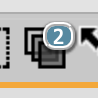
\includegraphics[width=0.45833in]{jira_imgs/3108.png}to bring up the
layers dialog, and enable the overlay of mask data:\\
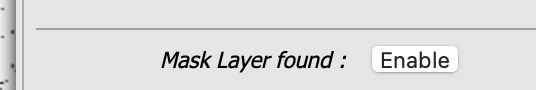
\includegraphics[width=3.12500in]{jira_imgs/3109.png}\\
Use the resulting dialog to request the overlay of one or more
individual mask planes.\\[2\baselineskip]Note that the mask plane colors
and transparency may be edited, and that the mask layer dialog also
highlights the mask status of the pixel currently at the mouse position.

}
\hdashrule[0.5ex]{\textwidth}{1pt}{3mm}
  Expected Result \\
{\footnotesize

}
\hdashrule[0.5ex]{\textwidth}{1pt}{3mm}
  Actual Result \\
{\footnotesize

}
\begin{tabular}{p{2cm}p{14cm}}
\toprule
Step 13 & Step Execution Status: \textbf{ Not Executed } \\ \hline
\end{tabular}
 Description \\
{\footnotesize
Dismiss the results of the previous search, by clicking on the ``x'' in
the ``tab'' atop the results table.\\
{{\\
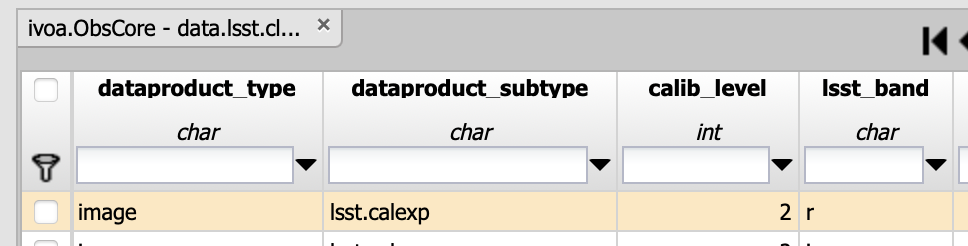
\includegraphics[width=1.56250in]{jira_imgs/3106.png}{Image Search
Results Table}}}

}
\hdashrule[0.5ex]{\textwidth}{1pt}{3mm}
  Expected Result \\
{\footnotesize

}
\hdashrule[0.5ex]{\textwidth}{1pt}{3mm}
  Actual Result \\
{\footnotesize

}
\begin{tabular}{p{2cm}p{14cm}}
\toprule
Step 14 & Step Execution Status: \textbf{ Not Executed } \\ \hline
\end{tabular}
 Description \\
{\footnotesize
If a calibration level is specified for this test, here: {(none)}⁠\\
ensure that the ``Observation Type and Source'' checkbox is selected,
and then check off the specified calibration level. ~Otherwise, ensure
that no calibration level is checked.

}
\hdashrule[0.5ex]{\textwidth}{1pt}{3mm}
  Expected Result \\
{\footnotesize

}
\hdashrule[0.5ex]{\textwidth}{1pt}{3mm}
  Actual Result \\
{\footnotesize

}
\begin{tabular}{p{2cm}p{14cm}}
\toprule
Step 15 & Step Execution Status: \textbf{ Not Executed } \\ \hline
\end{tabular}
 Description \\
{\footnotesize
Starting from the ObsTAP search screen, ensure that ``Location'' search
is unselected (using the checkbox). ~Ensure that ``Timing'' searches are
selected and that the disclosure triangle for their search specification
is opened (i.e., pointing down).\\[2\baselineskip]The specified time or
time range for this search is: {2024-10-01 00:00Z through 2024-11-01
00:00Z}⁠\\[2\baselineskip]Depending on the above value, select the
appropriate ``Time of Observation'' menu item: ``Completed in the last
\ldots{}'' for a relative time-since specification, or ``Overlapping
specified range'' for an absolute-time range. For the latter, select
``UTC date/times (ISO format)'' or ``MJD'' as appropriate to the way the
specification appears above. Type \textless{}TAB\textgreater{} or
otherwise leave the entry field.

}
\hdashrule[0.5ex]{\textwidth}{1pt}{3mm}
  Expected Result \\
{\footnotesize
The data entry fields in the ``Timing'' section of the screen should not
show any error (i.e., should not be highlighted in red).

}
\hdashrule[0.5ex]{\textwidth}{1pt}{3mm}
  Actual Result \\
{\footnotesize

}
\begin{tabular}{p{2cm}p{14cm}}
\toprule
Step 16 & Step Execution Status: \textbf{ Not Executed } \\ \hline
\end{tabular}
 Description \\
{\footnotesize
Limit the search to a specific detector: in the right-hand side of the
ObsTAP interface, enter the text below in order to do this. ~Then
execute the search. ~(NB: detector 94 happens to be the central CCD in
the array.)

}
\hdashrule[0.5ex]{\textwidth}{1pt}{3mm}
  Test Data \\
 {\footnotesize
=94

}
\hdashrule[0.5ex]{\textwidth}{1pt}{3mm}
  Expected Result \\
{\footnotesize
The result should be a table of observations for the specified date
range and the specified detector. ~Because no calibration level
restriction was applied, the search result should include multiple image
types.

}
\hdashrule[0.5ex]{\textwidth}{1pt}{3mm}
  Actual Result \\
{\footnotesize

}
\begin{tabular}{p{2cm}p{14cm}}
\toprule
Step 17 & Step Execution Status: \textbf{ Not Executed } \\ \hline
\end{tabular}
 Description \\
{\footnotesize
Verify by inspecting the dataproduct\_subtype column of the search
result that raw (lsst.raw), PVI (lsst.calexp), and difference images
(lsst.goodSeeingDiff\_differenceExp) are available. ~Verify by clicking
on rows of each type that each type of image can be displayed. ~Note in
particular that raw images have a different format (16 single-amplifier
images).

}
\hdashrule[0.5ex]{\textwidth}{1pt}{3mm}
  Expected Result \\
{\footnotesize

}
\hdashrule[0.5ex]{\textwidth}{1pt}{3mm}
  Actual Result \\
{\footnotesize

}
\begin{tabular}{p{2cm}p{14cm}}
\toprule
Step 18 & Step Execution Status: \textbf{ Not Executed } \\ \hline
\end{tabular}
 Description \\
{\footnotesize
Using the ability to sort the image metadata table by the ``t\_min''
column, select the earliest ``lsst.calexp'' image for the selected
detector in the query result.\\[2\baselineskip]Record, for concreteness,
the t\_min, lsst\_band, lsst\_visit, lsst\_detector, and obs\_id for
this row in the table.\\[2\baselineskip]In the single-image display
(``Data Product'' tab) for this image, click on the ``Pin Image''
button. ~This saves the image for further inspection. ~This is not
actually a pre-requisite for the actions that follow, but simplifies the
test conditions, for concreteness.

}
\hdashrule[0.5ex]{\textwidth}{1pt}{3mm}
  Expected Result \\
{\footnotesize

}
\hdashrule[0.5ex]{\textwidth}{1pt}{3mm}
  Actual Result \\
{\footnotesize

}
\begin{tabular}{p{2cm}p{14cm}}
\toprule
Step 19 & Step Execution Status: \textbf{ Not Executed } \\ \hline
\end{tabular}
 Description \\
{\footnotesize
Dismiss the results of the ObsTAP search, by clicking on the ``x'' in
the ``tab'' atop the results table.\\
{{\\
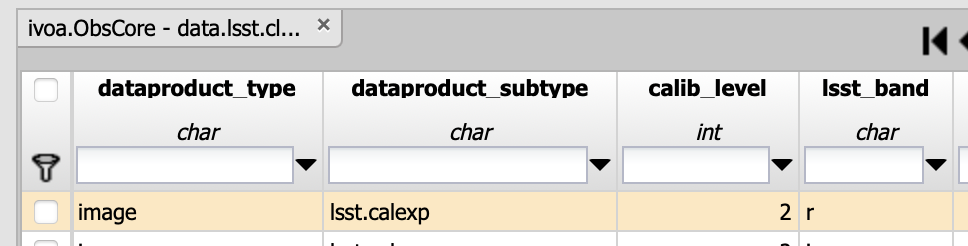
\includegraphics[width=1.56250in]{jira_imgs/3106.png}{Image Search
Results Table}}}

}
\hdashrule[0.5ex]{\textwidth}{1pt}{3mm}
  Expected Result \\
{\footnotesize
This should leave only the previously ``pinned'' image being displayed.

}
\hdashrule[0.5ex]{\textwidth}{1pt}{3mm}
  Actual Result \\
{\footnotesize

}
\begin{tabular}{p{2cm}p{14cm}}
\toprule
Step 20 & Step Execution Status: \textbf{ Not Executed } \\ \hline
\end{tabular}
 Description \\
{\footnotesize
Use the ``diskette'' button in the image toolbar to ``Save''/download
the image to a local FITS
file.\\[2\baselineskip]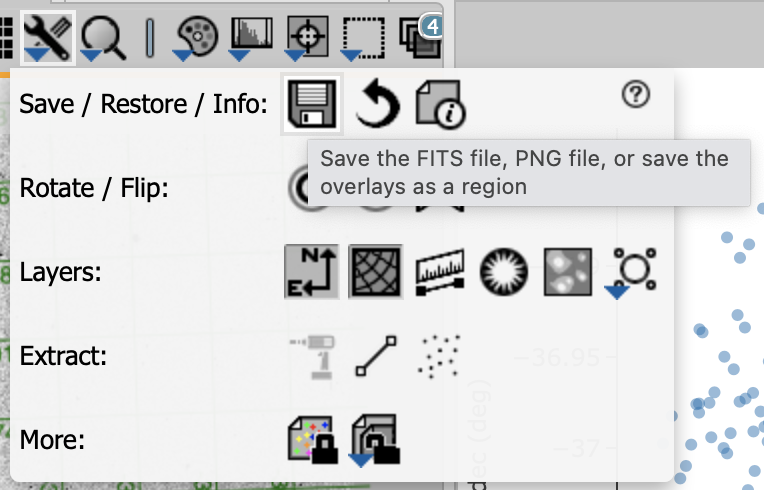
\includegraphics[width=3.12500in]{jira_imgs/3133.png}

}
\hdashrule[0.5ex]{\textwidth}{1pt}{3mm}
  Expected Result \\
{\footnotesize
A FITS file should be visible in the browser's download list.

}
\hdashrule[0.5ex]{\textwidth}{1pt}{3mm}
  Actual Result \\
{\footnotesize

}
\begin{tabular}{p{2cm}p{14cm}}
\toprule
Step 21 & Step Execution Status: \textbf{ Not Executed } \\ \hline
\end{tabular}
 Description \\
{\footnotesize
Use a non-Rubin tool to confirm that the file is in FITS format. ~Report
the tool used and any validation errors obtained - however, note that
Rubin does use some extensions and that the validation is not required
to be completely ``clean''.\\[2\baselineskip]A later version of this
test will be more explicit about what tool to use and what is an
acceptable deviation.

}
\hdashrule[0.5ex]{\textwidth}{1pt}{3mm}
  Expected Result \\
{\footnotesize

}
\hdashrule[0.5ex]{\textwidth}{1pt}{3mm}
  Actual Result \\
{\footnotesize

}
\begin{tabular}{p{2cm}p{14cm}}
\toprule
Step 22 & Step Execution Status: \textbf{ Not Executed } \\ \hline
\end{tabular}
 Description \\
{\footnotesize
Use the ``Info'' button in the image toolbar to display the FITS
headers.\\
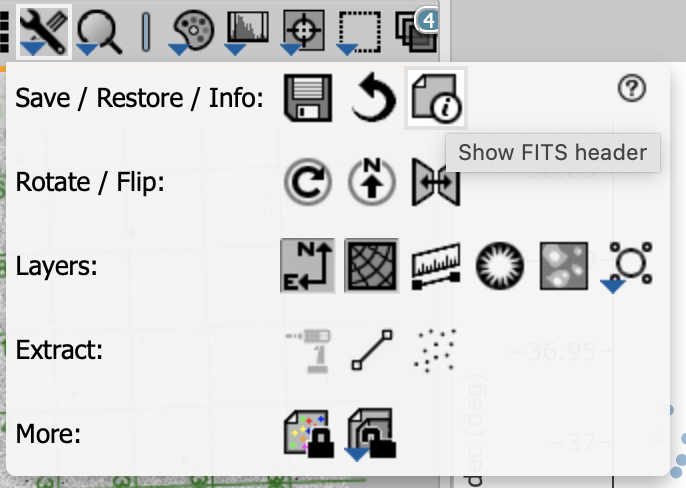
\includegraphics[width=3.12500in]{jira_imgs/3134.png}

}
\hdashrule[0.5ex]{\textwidth}{1pt}{3mm}
  Expected Result \\
{\footnotesize

}
\hdashrule[0.5ex]{\textwidth}{1pt}{3mm}
  Actual Result \\
{\footnotesize

}
\begin{tabular}{p{2cm}p{14cm}}
\toprule
Step 23 & Step Execution Status: \textbf{ Not Executed } \\ \hline
\end{tabular}
 Description \\
{\footnotesize
Click on the coordinate display name in the lower left of the image
pane. ~(This will likely initially say ``EQ-J2000''.) ~Record all
coordinate systems offered for the readout. ~Select ``Equatorial J2000
decimal''. ~Note that ``0-based pixel'' readout in fact respects the
LSST ``XY0'' convention, when present in the data, and will correctly
display offset coordinates, as for a patch within a
tract.\\[2\baselineskip]Click on the ``Show expanded readout \ldots{}''
button in the lower left. Configure the resulting display to show both
astrophysical and 0-based pixel coordinates.\\[2\baselineskip]Mouse
around in the image to explore the results.

}
\hdashrule[0.5ex]{\textwidth}{1pt}{3mm}
  Expected Result \\
{\footnotesize

}
\hdashrule[0.5ex]{\textwidth}{1pt}{3mm}
  Actual Result \\
{\footnotesize

}
\begin{tabular}{p{2cm}p{14cm}}
\toprule
Step 24 & Step Execution Status: \textbf{ Not Executed } \\ \hline
\end{tabular}
 Description \\
{\footnotesize
Click on ``lock by click'' and observe that the mode changes from
follow-mouse to retaining coordinate values for a selected point in the
image.\\[2\baselineskip]Use the provided copy-to-clipboard function\\
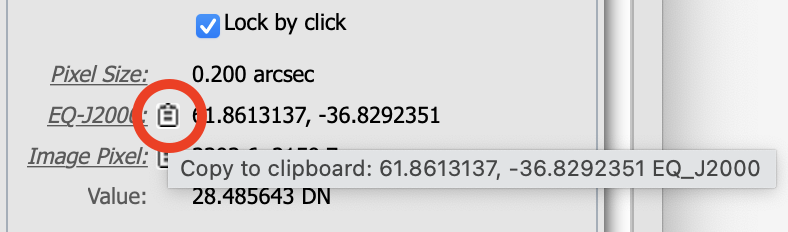
\includegraphics[width=3.12500in]{jira_imgs/3135.png}~and record the
resulting clipboard text.

}
\hdashrule[0.5ex]{\textwidth}{1pt}{3mm}
  Expected Result \\
{\footnotesize


}
\hdashrule[0.5ex]{\textwidth}{1pt}{3mm}
  Actual Result \\
{\footnotesize

}
\begin{tabular}{p{2cm}p{14cm}}
\toprule
Step 25 & Step Execution Status: \textbf{ Not Executed } \\ \hline
\end{tabular}
 Description \\
{\footnotesize
Confirm that, when the mouse is not rapidly moving, the pixel value is
displayed along with the coordinates.

}
\hdashrule[0.5ex]{\textwidth}{1pt}{3mm}
  Expected Result \\
{\footnotesize

}
\hdashrule[0.5ex]{\textwidth}{1pt}{3mm}
  Actual Result \\
{\footnotesize

}
\begin{tabular}{p{2cm}p{14cm}}
\toprule
Step 26 & Step Execution Status: \textbf{ Not Executed } \\ \hline
\end{tabular}
 Description \\
{\footnotesize
Using the corresponding image toolbar buttons, confirm that a
``compass'' (with the appropriate handedness) and a coordinate grid
overlay are available. ~\\[2\baselineskip]Compass:\\
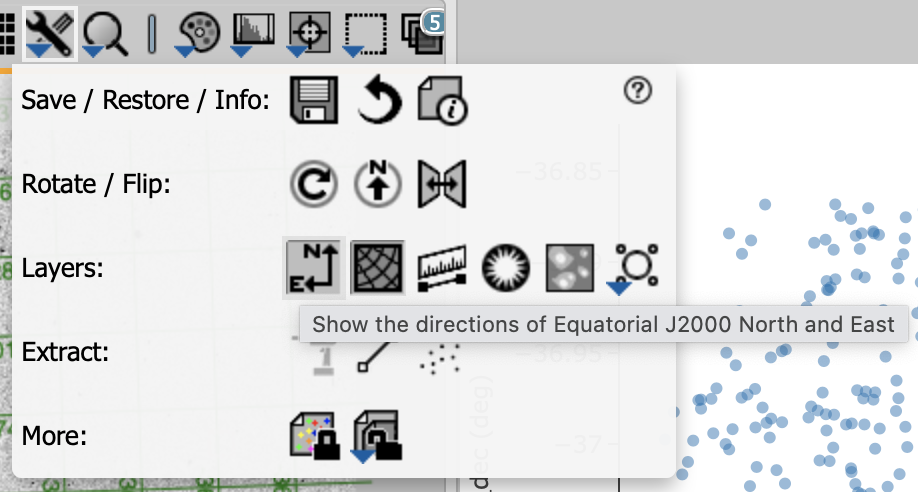
\includegraphics[width=3.12500in]{jira_imgs/3136.png}\\
Grid:\\
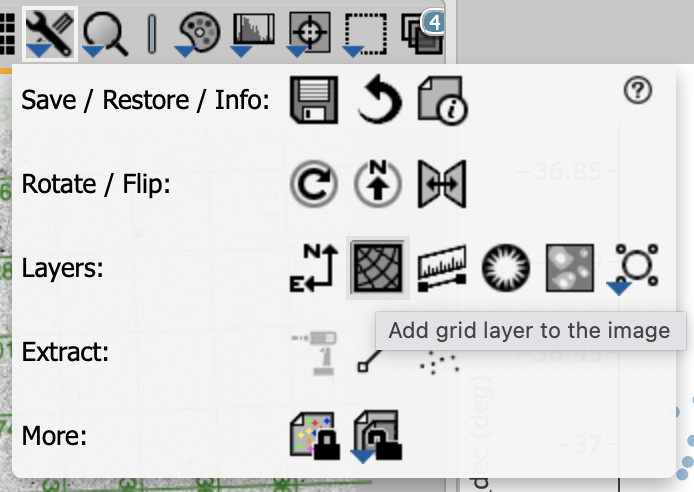
\includegraphics[width=3.12500in]{jira_imgs/3137.png}\\
With the grid displayed, use the layer-control dialog\\
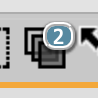
\includegraphics[width=0.33333in]{jira_imgs/3163.png} to explore the
different coordinate systems available, and record
them.\\[2\baselineskip]Then remove these overlays (using ``delete''
actions in the layer-control dialog) to avoid clutter in following
steps.

}
\hdashrule[0.5ex]{\textwidth}{1pt}{3mm}
  Expected Result \\
{\footnotesize

}
\hdashrule[0.5ex]{\textwidth}{1pt}{3mm}
  Actual Result \\
{\footnotesize

}
\begin{tabular}{p{2cm}p{14cm}}
\toprule
Step 27 & Step Execution Status: \textbf{ Not Executed } \\ \hline
\end{tabular}
 Description \\
{\footnotesize
Activate the distance-measurement tool using its image toolbar button.\\
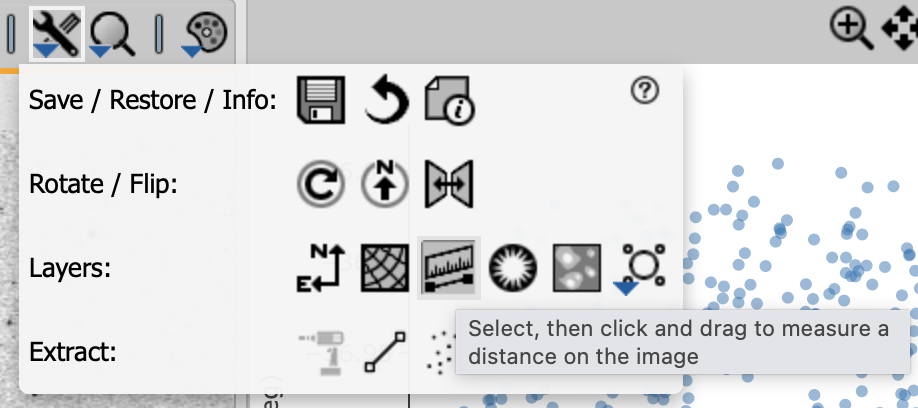
\includegraphics[width=3.12500in]{jira_imgs/3138.png}\\
Verify that it functions with both pixel and astrophysical distances and
gives plausible results. Use the layer-control dialog to explore the
ability to change the units of measurement.\\[2\baselineskip]For this
test it is not necessary to validate the distance calculation in detail.
A separate test case will perform a detailed comparison of an afw-based
measurement and a Portal measurement (see
DM-36236).\\[2\baselineskip]Again, to avoid clutter, use the
layer-control dialog to dismiss the distance-measurement tool.

}
\hdashrule[0.5ex]{\textwidth}{1pt}{3mm}
  Expected Result \\
{\footnotesize

}
\hdashrule[0.5ex]{\textwidth}{1pt}{3mm}
  Actual Result \\
{\footnotesize

}
\begin{tabular}{p{2cm}p{14cm}}
\toprule
Step 28 & Step Execution Status: \textbf{ Not Executed } \\ \hline
\end{tabular}
 Description \\
{\footnotesize
Use the ``rectangular selection'' tool to choose a subregion of the
displayed image.\\
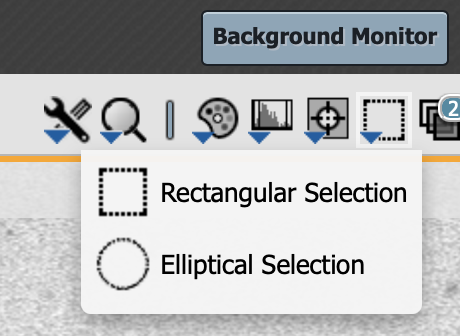
\includegraphics[width=3.12500in]{jira_imgs/3164.png}\\
Use the ``statistics'' button which appears in the image toolbar to
bring up an image-statistics dialog.\\
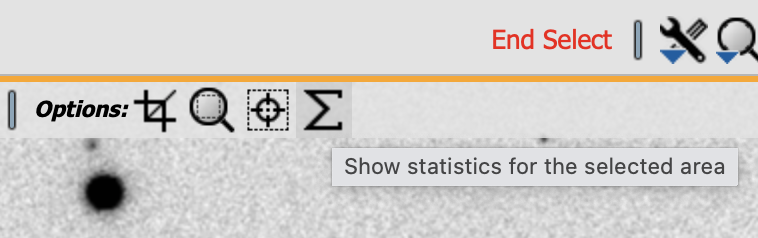
\includegraphics[width=3.12500in]{jira_imgs/3165.png}\\
Record a screenshot of the dialog and comment on the functionality
compared to the requirement.\\[2\baselineskip]Note that hovering over
the reported positions in the dialog results in their being highlighted
on the image.

}
\hdashrule[0.5ex]{\textwidth}{1pt}{3mm}
  Expected Result \\
{\footnotesize

}
\hdashrule[0.5ex]{\textwidth}{1pt}{3mm}
  Actual Result \\
{\footnotesize

}
\begin{tabular}{p{2cm}p{14cm}}
\toprule
Step 29 & Step Execution Status: \textbf{ Not Executed } \\ \hline
\end{tabular}
 Description \\
{\footnotesize
Use the image manipulation entries on the toolbar to modify the image
display. ~Comment on the behavior.\\[2\baselineskip]Use the ``Save''
button to confirm that it is possible to save a snapshot of the current
state as a PNG. Use this to document some samples of the
behavior.\\[2\baselineskip]It is not necessary to validate the actual
stretch algorithms in this test case, but a future test case should
address this.

}
\hdashrule[0.5ex]{\textwidth}{1pt}{3mm}
  Expected Result \\
{\footnotesize

}
\hdashrule[0.5ex]{\textwidth}{1pt}{3mm}
  Actual Result \\
{\footnotesize

}
\begin{tabular}{p{2cm}p{14cm}}
\toprule
Step 30 & Step Execution Status: \textbf{ Not Executed } \\ \hline
\end{tabular}
 Description \\
{\footnotesize
Confirm that it is possible to pan, zoom, and rotate an image, and to
save-as-PNG to save the results.

}
\hdashrule[0.5ex]{\textwidth}{1pt}{3mm}
  Expected Result \\
{\footnotesize

}
\hdashrule[0.5ex]{\textwidth}{1pt}{3mm}
  Actual Result \\
{\footnotesize

}
\begin{tabular}{p{2cm}p{14cm}}
\toprule
Step 31 & Step Execution Status: \textbf{ Not Executed } \\ \hline
\end{tabular}
 Description \\
{\footnotesize
Close the Portal window and open a new one. ~Re-authentication should
not be necessary unless using a private window.\\[2\baselineskip]Again,
this is not required but keeps the test conditions from accumulating
residue of previous steps.

}
\hdashrule[0.5ex]{\textwidth}{1pt}{3mm}
  Expected Result \\
{\footnotesize

}
\hdashrule[0.5ex]{\textwidth}{1pt}{3mm}
  Actual Result \\
{\footnotesize

}
\begin{tabular}{p{2cm}p{14cm}}
\toprule
Step 32 & Step Execution Status: \textbf{ Not Executed } \\ \hline
\end{tabular}
 Description \\
{\footnotesize
If a calibration level is specified for this test, here: {2}⁠~\\
ensure that the ``Observation Type and Source'' checkbox is selected,
and then check off the specified calibration level. Otherwise, ensure
that no calibration level is checked.

}
\hdashrule[0.5ex]{\textwidth}{1pt}{3mm}
  Expected Result \\
{\footnotesize

}
\hdashrule[0.5ex]{\textwidth}{1pt}{3mm}
  Actual Result \\
{\footnotesize

}
\begin{tabular}{p{2cm}p{14cm}}
\toprule
Step 33 & Step Execution Status: \textbf{ Not Executed } \\ \hline
\end{tabular}
 Description \\
{\footnotesize
Ensure that the ``Location'' and ``Timing'' selectors on the ObsTAP
screen are unchecked. ~(These will be implicit in the Visit ID.)

}
\hdashrule[0.5ex]{\textwidth}{1pt}{3mm}
  Expected Result \\
{\footnotesize

}
\hdashrule[0.5ex]{\textwidth}{1pt}{3mm}
  Actual Result \\
{\footnotesize

}
\begin{tabular}{p{2cm}p{14cm}}
\toprule
Step 34 & Step Execution Status: \textbf{ Not Executed } \\ \hline
\end{tabular}
 Description \\
{\footnotesize
Enter the Visit ID, {538450}⁠ , as a constraint on the ``lsst\_visit''
field in the constraints table on the right side of the UI, as "=
{538450}⁠ ".

}
\hdashrule[0.5ex]{\textwidth}{1pt}{3mm}
  Expected Result \\
{\footnotesize

}
\hdashrule[0.5ex]{\textwidth}{1pt}{3mm}
  Actual Result \\
{\footnotesize

}
\begin{tabular}{p{2cm}p{14cm}}
\toprule
Step 35 & Step Execution Status: \textbf{ Not Executed } \\ \hline
\end{tabular}
 Description \\
{\footnotesize
Execute the search.

}
\hdashrule[0.5ex]{\textwidth}{1pt}{3mm}
  Expected Result \\
{\footnotesize
The usual Portal ``tri-view'' should appear, with a table of all the
CCD-level images in the selected visit in the bottom half of the
display, coverage map and single-image-display tabs in the upper left,
and an X-Y plot in the upper right.

}
\hdashrule[0.5ex]{\textwidth}{1pt}{3mm}
  Actual Result \\
{\footnotesize

}
\begin{tabular}{p{2cm}p{14cm}}
\toprule
Step 36 & Step Execution Status: \textbf{ Not Executed } \\ \hline
\end{tabular}
 Description \\
{\footnotesize
Verify that clicking on rows in the table, image frames in the coverage
plot, and points in the X-Y plot all take effect across all three views,
and change which image is actually displayed.

}
\hdashrule[0.5ex]{\textwidth}{1pt}{3mm}
  Expected Result \\
{\footnotesize

}
\hdashrule[0.5ex]{\textwidth}{1pt}{3mm}
  Actual Result \\
{\footnotesize

}
\begin{tabular}{p{2cm}p{14cm}}
\toprule
Step 37 & Step Execution Status: \textbf{ Not Executed } \\ \hline
\end{tabular}
 Description \\
{\footnotesize
Verify that the coverage image displays the expected pattern of CCDs in
the focal plane for a single visit, projected on the sky.

}
\hdashrule[0.5ex]{\textwidth}{1pt}{3mm}
  Expected Result \\
{\footnotesize

}
\hdashrule[0.5ex]{\textwidth}{1pt}{3mm}
  Actual Result \\
{\footnotesize

}
\begin{tabular}{p{2cm}p{14cm}}
\toprule
Step 38 & Step Execution Status: \textbf{ Not Executed } \\ \hline
\end{tabular}
 Description \\
{\footnotesize
Verify that the correct visit was returned.

}
\hdashrule[0.5ex]{\textwidth}{1pt}{3mm}
  Expected Result \\
{\footnotesize

}
\hdashrule[0.5ex]{\textwidth}{1pt}{3mm}
  Actual Result \\
{\footnotesize

}
\begin{tabular}{p{2cm}p{14cm}}
\toprule
Step 39 & Step Execution Status: \textbf{ Not Executed } \\ \hline
\end{tabular}
 Description \\
{\footnotesize
This step confirms that the image search was done via an ADQL (ObsTAP)
search in the Portal Aspect.\\[2\baselineskip]Click on the ``(i)''
button in the image metadata table toolbar. From the resulting dialog,
record the ``Job Link'', using the copy-to-clipboard button provided.
Note that it is under the API-Aspect endpoint of the RSP instance under
test.\\[2\baselineskip]Click on the ``Job Link'' URL in the dialog. ~A
browser window containing the XML job definition will appear. ~Save the
XML and attach it to this test. ~Extract the ADQL text from the
`\textless{}uws:parameter id=``QUERY''\textgreater{}' element in the XML
and record it.

}
\hdashrule[0.5ex]{\textwidth}{1pt}{3mm}
  Expected Result \\
{\footnotesize

}
\hdashrule[0.5ex]{\textwidth}{1pt}{3mm}
  Actual Result \\
{\footnotesize

}
\begin{tabular}{p{2cm}p{14cm}}
\toprule
Step 40 & Step Execution Status: \textbf{ Not Executed } \\ \hline
\end{tabular}
 Description \\
{\footnotesize
Use the ``RSP TAP Search'' screen to perform a search on the
dp02\_dc2\_catalogs.Visit table for visit {538450}⁠ :

\begin{enumerate}
\tightlist
\item
  Unselect both the ``Spatial'' and ``Temporal'' constraint tools on the
  left side of section 4, ``Enter Constraints''.
\item
  On the right side, enter "= {538450}⁠ " in the ``Constraints'' field
  in the table for the ``visit'' attribute.
\item
  Execute the search.
\end{enumerate}

Record the number of rows returned and describe the data.

}
\hdashrule[0.5ex]{\textwidth}{1pt}{3mm}
  Expected Result \\
{\footnotesize
A single-row table should be returned with high-level metadata for the
full visit.

}
\hdashrule[0.5ex]{\textwidth}{1pt}{3mm}
  Actual Result \\
{\footnotesize

}
\begin{tabular}{p{2cm}p{14cm}}
\toprule
Step 41 & Step Execution Status: \textbf{ Not Executed } \\ \hline
\end{tabular}
 Description \\
{\footnotesize
Use the ``RSP TAP Search'' screen to perform a search on the
dp02\_dc2\_catalogs.CcdVisit table for visit {538450}⁠ :

\begin{enumerate}
\tightlist
\item
  Unselect both the ``Spatial'' and ``Temporal'' constraint tools on the
  left side of section 4, ``Enter Constraints''.
\item
  On the right side, enter "= {538450}⁠ " in the ``Constraints'' field
  in the table for the ``visitId'' attribute.
\item
  Execute the search.
\end{enumerate}

Record the number of rows returned and describe the
data.\\[2\baselineskip]Note whether the observation time varies per-CCD
as it should for real data. ~However, that is not germane to the
test-passing criteria; it is a Science Pipelines issue.

}
\hdashrule[0.5ex]{\textwidth}{1pt}{3mm}
  Expected Result \\
{\footnotesize
A 189-row table should be returned with per-CCD metadata on the result
of the data processing.

}
\hdashrule[0.5ex]{\textwidth}{1pt}{3mm}
  Actual Result \\
{\footnotesize

}

\paragraph{ LVV-T2721 - LDM-503-RSPa: Portal Aspect tests for DP0.2 readiness - coadded images }\mbox{}\\

Version \textbf{1}.
Open  \href{https://jira.lsstcorp.org/secure/Tests.jspa#/testCase/LVV-T2721}{\textit{ LVV-T2721 } }
test case in Jira.

Verify that the subset of RSP Portal capabilities planned to be added
for DP0.2 are present, as pertaining to coadded images

\textbf{ Preconditions}:\\


Execution status: {\bf Not Executed }

Final comment:\\


Detailed steps results:

\begin{tabular}{p{2cm}p{14cm}}
\toprule
Step 1 & Step Execution Status: \textbf{ Not Executed } \\ \hline
\end{tabular}
 Description \\
{\footnotesize
Navigate to the Portal Aspect endpoint. ~The stable version of the RSP
at the interim data facility (IDF) should be used for this test and is
currently located at: \url{https://data.lsst.cloud/}. The Portal Aspect
can be reached by clicking on ``Portal'' in the RSP home page or by
navigating directly to~\url{https://data.lsst.cloud/portal/app}.

}
\hdashrule[0.5ex]{\textwidth}{1pt}{3mm}
  Expected Result \\
{\footnotesize
A credential-entry screen should be displayed.

}
\hdashrule[0.5ex]{\textwidth}{1pt}{3mm}
  Actual Result \\
{\footnotesize

}
\begin{tabular}{p{2cm}p{14cm}}
\toprule
Step 2 & Step Execution Status: \textbf{ Not Executed } \\ \hline
\end{tabular}
 Description \\
{\footnotesize
Enter a valid set of credentials for an LSST user with RSP access on the
instance under test.

}
\hdashrule[0.5ex]{\textwidth}{1pt}{3mm}
  Expected Result \\
{\footnotesize
The Portal Aspect UI should be displayed following authentication.

}
\hdashrule[0.5ex]{\textwidth}{1pt}{3mm}
  Actual Result \\
{\footnotesize

}
\begin{tabular}{p{2cm}p{14cm}}
\toprule
Step 3 & Step Execution Status: \textbf{ Not Executed } \\ \hline
\end{tabular}
 Description \\
{\footnotesize
Within the Portal Aspect UI, navigate, if necessary, to the ``RSP Tap
Search'' screen, using the ``blue button'' at the top left of the Portal
Aspect UI.

}
\hdashrule[0.5ex]{\textwidth}{1pt}{3mm}
  Expected Result \\
{\footnotesize
A screen titled ``TAP Searches'' is displayed.

}
\hdashrule[0.5ex]{\textwidth}{1pt}{3mm}
  Actual Result \\
{\footnotesize

}
\begin{tabular}{p{2cm}p{14cm}}
\toprule
Step 4 & Step Execution Status: \textbf{ Not Executed } \\ \hline
\end{tabular}
 Description \\
{\footnotesize
Ensure that the RSP instance's own TAP service is selected in Section 1
of the screen.

}
\hdashrule[0.5ex]{\textwidth}{1pt}{3mm}
  Expected Result \\
{\footnotesize
The ``Select TAP Service'' menu should be displaying ``Using LSST RSP''.

}
\hdashrule[0.5ex]{\textwidth}{1pt}{3mm}
  Actual Result \\
{\footnotesize

}
\begin{tabular}{p{2cm}p{14cm}}
\toprule
Step 5 & Step Execution Status: \textbf{ Not Executed } \\ \hline
\end{tabular}
 Description \\
{\footnotesize
Select ``Image Search (ObsTAP)'' in Section 2 of the screen.

}
\hdashrule[0.5ex]{\textwidth}{1pt}{3mm}
  Expected Result \\
{\footnotesize
The screen should change to show ``(Searching the ivoa.ObsCore table on
this service\ldots{})'' in Section 2 and to display~a Section 3
beginning with an ``Observation Type and Source'' selector.

}
\hdashrule[0.5ex]{\textwidth}{1pt}{3mm}
  Actual Result \\
{\footnotesize

}
\begin{tabular}{p{2cm}p{14cm}}
\toprule
Step 6 & Step Execution Status: \textbf{ Not Executed } \\ \hline
\end{tabular}
 Description \\
{\footnotesize
If a calibration level is specified for this test, here: {3}⁠\\
ensure that the ``Observation Type and Source'' checkbox is selected,
and then check off the specified calibration level. ~Otherwise, ensure
that no calibration level is checked.

}
\hdashrule[0.5ex]{\textwidth}{1pt}{3mm}
  Expected Result \\
{\footnotesize

}
\hdashrule[0.5ex]{\textwidth}{1pt}{3mm}
  Actual Result \\
{\footnotesize

}
\begin{tabular}{p{2cm}p{14cm}}
\toprule
Step 7 & Step Execution Status: \textbf{ Not Executed } \\ \hline
\end{tabular}
 Description \\
{\footnotesize
Starting from the ObsTAP search screen, ensure that ``Location'' search
is selected (using the checkbox), and that the disclosure triangle for
its search specification is opened (i.e., pointing down).\\
Ensure that the query type ``Observation boundary contains point'' is
selected. Enter the target coordinates {62.0, -37.0}⁠ in the
``Coordinates or object name'' field. Type \textless{}TAB\textgreater{}
or otherwise leave the entry field.

}
\hdashrule[0.5ex]{\textwidth}{1pt}{3mm}
  Expected Result \\
{\footnotesize
The ``Coordinates of object name'' field should not show an error (i.e.,
should not be highlighted in red).

}
\hdashrule[0.5ex]{\textwidth}{1pt}{3mm}
  Actual Result \\
{\footnotesize

}
\begin{tabular}{p{2cm}p{14cm}}
\toprule
Step 8 & Step Execution Status: \textbf{ Not Executed } \\ \hline
\end{tabular}
 Description \\
{\footnotesize
Observe and report on the absence of an obvious way to say ``I only want
to see coadds''. ~This is a known weakness of relying on the ObsCore
data model exclusively; there's no unambiguous way in ObsCore to express
such a limitation on a search.\\[2\baselineskip]Calibration level 3,
chosen above, selects derived images, but unfortunately for this purpose
that includes both single-epoch difference images and multi-epoch
coadds.\\[2\baselineskip]It would be possible to select on t\_exptime,
to ask for effective exposure times (much) longer than the single-epoch
norm of 30 seconds, but unfortunately at this time the pipelines don't
report even an approximate exposure time for coadds.\\[2\baselineskip]A
forthcoming version of the Portal will be pre-configured with a pick
list of the available image types, which will address this need, but in
the mean time, the next test step provides a
workaround.\\[2\baselineskip](This test case will be updated once it is
available.)

}
\hdashrule[0.5ex]{\textwidth}{1pt}{3mm}
  Expected Result \\
{\footnotesize

}
\hdashrule[0.5ex]{\textwidth}{1pt}{3mm}
  Actual Result \\
{\footnotesize

}
\begin{tabular}{p{2cm}p{14cm}}
\toprule
Step 9 & Step Execution Status: \textbf{ Not Executed } \\ \hline
\end{tabular}
 Description \\
{\footnotesize
Use the constraints table on the right of the search screen to add the
constraint ``\textgreater{}0'' to the ``lsst\_tract'' field. ~This
requires the images selected by the search to have an assigned location
in the coadded skymap, effectively selecting coadds.\\[2\baselineskip]As
noted above, this is a workaround and is not the intended final UX.

}
\hdashrule[0.5ex]{\textwidth}{1pt}{3mm}
  Expected Result \\
{\footnotesize

}
\hdashrule[0.5ex]{\textwidth}{1pt}{3mm}
  Actual Result \\
{\footnotesize

}
\begin{tabular}{p{2cm}p{14cm}}
\toprule
Step 10 & Step Execution Status: \textbf{ Not Executed } \\ \hline
\end{tabular}
 Description \\
{\footnotesize
Execute the search. ~Note the number of images returned. ~Note the
values of ``dataproduct\_subtype'' returned.

}
\hdashrule[0.5ex]{\textwidth}{1pt}{3mm}
  Expected Result \\
{\footnotesize
Following the execution of the search, the Portal Aspect should display,
in its standard table viewer, a list of 24 coadded images: from two
coadd ``patches'' that both happen to overlap the specified target, from
two types of coadds - ``deep'' and ``good seeing'', identified by
``dataproduct\_subtype'' values of ``lsst.deepCoadd\_calexp'' and
``lsst.goodSeeingCoadd'', respectively (strings derived directly from
the Butler dataset type of the images) - and from six filters; 2*2*6 =
24.\\[2\baselineskip]On the upper left there will be a pane with two
tabs: ``Coverage'', which should display the outline of the images on
the sky, and ``Data Product'', which should display the currently
selected image in the table.\\[2\baselineskip]On the upper right, there
will be an x-y plot of the central RA and Dec of each of the images.

}
\hdashrule[0.5ex]{\textwidth}{1pt}{3mm}
  Actual Result \\
{\footnotesize

}
\begin{tabular}{p{2cm}p{14cm}}
\toprule
Step 11 & Step Execution Status: \textbf{ Not Executed } \\ \hline
\end{tabular}
 Description \\
{\footnotesize
Verify that the result table contains information on the filter band,
both as the custom column ``lsst-band'' and as the ObsCore-standard
columns ``em\_min'' and ``em\_max''. ~Verify that it is possible to
narrow the selection by filter band using the table viewer's filtering
tools.

}
\hdashrule[0.5ex]{\textwidth}{1pt}{3mm}
  Expected Result \\
{\footnotesize

}
\hdashrule[0.5ex]{\textwidth}{1pt}{3mm}
  Actual Result \\
{\footnotesize

}
\begin{tabular}{p{2cm}p{14cm}}
\toprule
Step 12 & Step Execution Status: \textbf{ Not Executed } \\ \hline
\end{tabular}
 Description \\
{\footnotesize
Verify that clicking on rows in the table, points in the scatter plot,
and frames in the coverage image all serve to change the currently
displayed image and are reflected in all the panes in a coordinated way.

}
\hdashrule[0.5ex]{\textwidth}{1pt}{3mm}
  Expected Result \\
{\footnotesize
The ``linking'' behavior normal to Portal Aspect results displays should
be seen to apply equally well to image search results.

}
\hdashrule[0.5ex]{\textwidth}{1pt}{3mm}
  Actual Result \\
{\footnotesize

}
\begin{tabular}{p{2cm}p{14cm}}
\toprule
Step 13 & Step Execution Status: \textbf{ Not Executed } \\ \hline
\end{tabular}
 Description \\
{\footnotesize
For one of the selected images, verify, by using the select-extension
controls, that the mask and variance planes of the image can be
displayed.\\

\includegraphics[width=3.12500in]{jira_imgs/3107.png}\\
Use the ``image layers'' toolbar button\\
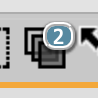
\includegraphics[width=0.45833in]{jira_imgs/3108.png}to bring up the
layers dialog, and enable the overlay of mask data:\\
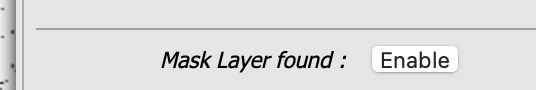
\includegraphics[width=3.12500in]{jira_imgs/3109.png}\\
Use the resulting dialog to request the overlay of one or more
individual mask planes.\\[2\baselineskip]Note that the mask plane colors
and transparency may be edited, and that the mask layer dialog also
highlights the mask status of the pixel currently at the mouse position.

}
\hdashrule[0.5ex]{\textwidth}{1pt}{3mm}
  Expected Result \\
{\footnotesize

}
\hdashrule[0.5ex]{\textwidth}{1pt}{3mm}
  Actual Result \\
{\footnotesize

}
\begin{tabular}{p{2cm}p{14cm}}
\toprule
Step 14 & Step Execution Status: \textbf{ Not Executed } \\ \hline
\end{tabular}
 Description \\
{\footnotesize
Dismiss the results of the previous search, by clicking on the ``x'' in
the ``tab'' atop the results table.\\
{{\\
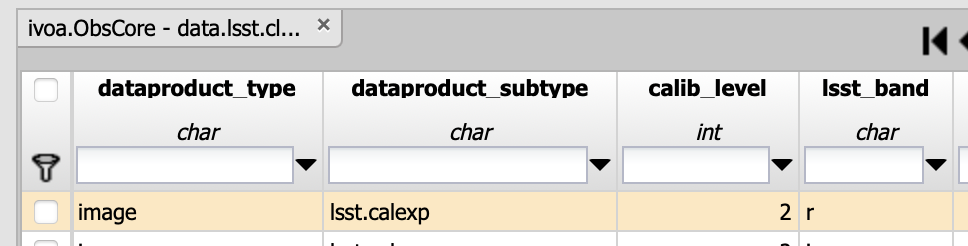
\includegraphics[width=1.56250in]{jira_imgs/3106.png}{Image Search
Results Table}}}

}
\hdashrule[0.5ex]{\textwidth}{1pt}{3mm}
  Expected Result \\
{\footnotesize

}
\hdashrule[0.5ex]{\textwidth}{1pt}{3mm}
  Actual Result \\
{\footnotesize

}

\paragraph{ LVV-T2716 - LDM-503-RSPa: Test HiPS functionality in DP0.2 }\mbox{}\\

Version \textbf{1}.
Open  \href{https://jira.lsstcorp.org/secure/Tests.jspa#/testCase/LVV-T2716}{\textit{ LVV-T2716 } }
test case in Jira.

Verify DM and RSP requirements on the availability of Rubin-created HiPS
imaging, within the context of DP0.2.

\textbf{ Preconditions}:\\


Execution status: {\bf Not Executed }

Final comment:\\


Detailed steps results:

\begin{tabular}{p{2cm}p{14cm}}
\toprule
Step 1 & Step Execution Status: \textbf{ Not Executed } \\ \hline
\end{tabular}
 Description \\
{\footnotesize
Navigate to the Portal Aspect endpoint. ~The stable version of the RSP
at the interim data facility (IDF) should be used for this test and is
currently located at: \url{https://data.lsst.cloud/}. The Portal Aspect
can be reached by clicking on ``Portal'' in the RSP home page or by
navigating directly to~\url{https://data.lsst.cloud/portal/app}.

}
\hdashrule[0.5ex]{\textwidth}{1pt}{3mm}
  Expected Result \\
{\footnotesize
A credential-entry screen should be displayed.

}
\hdashrule[0.5ex]{\textwidth}{1pt}{3mm}
  Actual Result \\
{\footnotesize

}
\begin{tabular}{p{2cm}p{14cm}}
\toprule
Step 2 & Step Execution Status: \textbf{ Not Executed } \\ \hline
\end{tabular}
 Description \\
{\footnotesize
Enter a valid set of credentials for an LSST user with RSP access on the
instance under test.

}
\hdashrule[0.5ex]{\textwidth}{1pt}{3mm}
  Expected Result \\
{\footnotesize
The Portal Aspect UI should be displayed following authentication.

}
\hdashrule[0.5ex]{\textwidth}{1pt}{3mm}
  Actual Result \\
{\footnotesize

}
\begin{tabular}{p{2cm}p{14cm}}
\toprule
Step 3 & Step Execution Status: \textbf{ Not Executed } \\ \hline
\end{tabular}
 Description \\
{\footnotesize
{Navigate to the ``External Images'' tab of the interface. ~This is a
temporary workaround - a more obvious path for this will be provided in
a future version of the Portal Aspect application.}

}
\hdashrule[0.5ex]{\textwidth}{1pt}{3mm}
  Expected Result \\
{\footnotesize

}
\hdashrule[0.5ex]{\textwidth}{1pt}{3mm}
  Actual Result \\
{\footnotesize

}
\begin{tabular}{p{2cm}p{14cm}}
\toprule
Step 4 & Step Execution Status: \textbf{ Not Executed } \\ \hline
\end{tabular}
 Description \\
{\footnotesize
In ``1. Choose Image Type'' select ``View HiPS Images''. ~Leave ``2.
Select Image Source'' and ``3. Select Target'' at their defaults
(``Search'', and empty data-entry fields,
respectively).\\[2\baselineskip]Record the HiPS images that are
displayed in the resulting pick list.

}
\hdashrule[0.5ex]{\textwidth}{1pt}{3mm}
  Expected Result \\
{\footnotesize
In ``4. Select Data Set'' a checkbox ``Rubin Featured'' should be
checked, and a list of seven or eight HiPS images from DP0.2 should be
displayed: six single-band images and one or more three-color images.

}
\hdashrule[0.5ex]{\textwidth}{1pt}{3mm}
  Actual Result \\
{\footnotesize

}
\begin{tabular}{p{2cm}p{14cm}}
\toprule
Step 5 & Step Execution Status: \textbf{ Not Executed } \\ \hline
\end{tabular}
 Description \\
{\footnotesize
Click on the ``(i)'' icon in one of the rows. ~Note the display of a
HiPS ``properties'' file in a new window. ~Record the full URL for this
window. ~Then close the window.\\[2\baselineskip]Verify that the URL
begins with ``https:''.\\[2\baselineskip]Verify that the URL cannot be
opened successfully in a private browser window. Record the error
indication received.

}
\hdashrule[0.5ex]{\textwidth}{1pt}{3mm}
  Expected Result \\
{\footnotesize
E.g., ``https://data.lsst.cloud/api/hips/images/band\_u/properties''.

}
\hdashrule[0.5ex]{\textwidth}{1pt}{3mm}
  Actual Result \\
{\footnotesize

}
\begin{tabular}{p{2cm}p{14cm}}
\toprule
Step 6 & Step Execution Status: \textbf{ Not Executed } \\ \hline
\end{tabular}
 Description \\
{\footnotesize
Select one of the HiPS images in the displayed table, and record the
selected map and its displayed pixel scale.\\[2\baselineskip]Click on
the ``Search'' button in the lower left of the UI. ~Record the time
required to put up an initial display of the image.

}
\hdashrule[0.5ex]{\textwidth}{1pt}{3mm}
  Expected Result \\
{\footnotesize
The HiPS image should be displayed.

}
\hdashrule[0.5ex]{\textwidth}{1pt}{3mm}
  Actual Result \\
{\footnotesize

}
\begin{tabular}{p{2cm}p{14cm}}
\toprule
Step 7 & Step Execution Status: \textbf{ Not Executed } \\ \hline
\end{tabular}
 Description \\
{\footnotesize
Verify that the UI permits panning and zooming on the image. ~Note the
limited coverage (roughly 300 sq. deg., less than 1\% of the sky) of the
map, so this is not a full test of the performance of these functions at
a zoomed-out scale.

}
\hdashrule[0.5ex]{\textwidth}{1pt}{3mm}
  Expected Result \\
{\footnotesize

}
\hdashrule[0.5ex]{\textwidth}{1pt}{3mm}
  Actual Result \\
{\footnotesize

}
\begin{tabular}{p{2cm}p{14cm}}
\toprule
Step 8 & Step Execution Status: \textbf{ Not Executed } \\ \hline
\end{tabular}
 Description \\
{\footnotesize
Verify that coordinate readouts are available for the mouse position on
the HiPS image. ~Record the available coordinate systems.

}
\hdashrule[0.5ex]{\textwidth}{1pt}{3mm}
  Expected Result \\
{\footnotesize

}
\hdashrule[0.5ex]{\textwidth}{1pt}{3mm}
  Actual Result \\
{\footnotesize

}
\begin{tabular}{p{2cm}p{14cm}}
\toprule
Step 9 & Step Execution Status: \textbf{ Not Executed } \\ \hline
\end{tabular}
 Description \\
{\footnotesize
Add the coordinate-lines overlay with the usual toolbar button:~\\
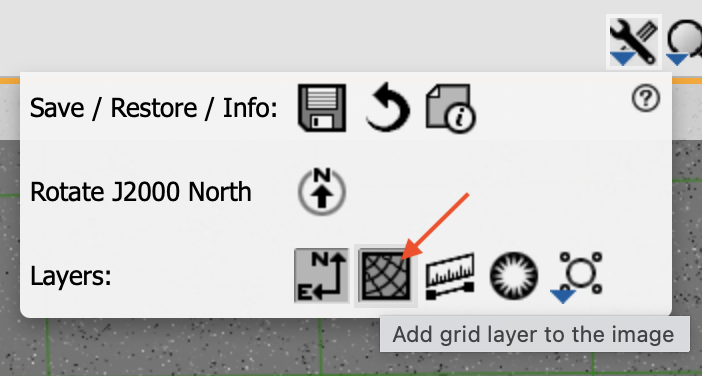
\includegraphics[width=3.12500in]{jira_imgs/3131.png}\\
Verify that the display accords roughly with the standard Portal Aspect
coordinate readout. ~Then use the layers dialog~\\
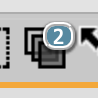
\includegraphics[width=0.44792in]{jira_imgs/3132.png}to delete the grid
overlay.

}
\hdashrule[0.5ex]{\textwidth}{1pt}{3mm}
  Expected Result \\
{\footnotesize

}
\hdashrule[0.5ex]{\textwidth}{1pt}{3mm}
  Actual Result \\
{\footnotesize

}
\begin{tabular}{p{2cm}p{14cm}}
\toprule
Step 10 & Step Execution Status: \textbf{ Not Executed } \\ \hline
\end{tabular}
 Description \\
{\footnotesize
If the selected HiPS image was the ``gri color'' one, change to one of
the single-band ones. ~Ensure that it behaves similarly. ~Leave it
selected.

}
\hdashrule[0.5ex]{\textwidth}{1pt}{3mm}
  Expected Result \\
{\footnotesize

}
\hdashrule[0.5ex]{\textwidth}{1pt}{3mm}
  Actual Result \\
{\footnotesize

}
\begin{tabular}{p{2cm}p{14cm}}
\toprule
Step 11 & Step Execution Status: \textbf{ Not Executed } \\ \hline
\end{tabular}
 Description \\
{\footnotesize
Navigate to the ``RSP TAP Search'' screen in the Portal. Select the
``Single Table'' query type.

}
\hdashrule[0.5ex]{\textwidth}{1pt}{3mm}
  Expected Result \\
{\footnotesize

}
\hdashrule[0.5ex]{\textwidth}{1pt}{3mm}
  Actual Result \\
{\footnotesize

}
\begin{tabular}{p{2cm}p{14cm}}
\toprule
Step 12 & Step Execution Status: \textbf{ Not Executed } \\ \hline
\end{tabular}
 Description \\
{\footnotesize
Select the " {dp02\_dc2\_catalogs}⁠ " table collection/schema and the "
{Object}⁠ " table.

}
\hdashrule[0.5ex]{\textwidth}{1pt}{3mm}
  Expected Result \\
{\footnotesize

}
\hdashrule[0.5ex]{\textwidth}{1pt}{3mm}
  Actual Result \\
{\footnotesize

}
\begin{tabular}{p{2cm}p{14cm}}
\toprule
Step 13 & Step Execution Status: \textbf{ Not Executed } \\ \hline
\end{tabular}
 Description \\
{\footnotesize
Verify that queries in Galactic and Ecliptic coordinate systems are
possible:\\[2\baselineskip]

\begin{enumerate}
\tightlist
\item
  Enter a search radius of 0.02 degrees.
\item
  Enter the target coordinates ``239.143686, -47.681348 gal''
  (Galactic). ~Use the ``Populate and edit ADQL'' button at the bottom
  of the screen to inspect the resulting ADQL for the CIRCLE construct,
  which should be in ICRS degrees. ~Verify that it is close to (62.0,
  -37.0) in those units. ~Return to the ``Single Table'' search screen.
\item
  Enter the target coordinates ``47.388563, -56.371758 ecl'' (ecliptic).
  ~Use the ``Populate and edit ADQL'' button at the bottom of the screen
  to inspect the resulting ADQL for the CIRCLE construct, which should
  be in ICRS degrees. ~Verify that it is close to (62.0, -37.0) in those
  units. ~Return to the ``Single Table'' search screen.
\end{enumerate}

}
\hdashrule[0.5ex]{\textwidth}{1pt}{3mm}
  Expected Result \\
{\footnotesize
E.g., CIRCLE('ICRS', 61.9999155538758, -36.99994564119228, 0.02)

}
\hdashrule[0.5ex]{\textwidth}{1pt}{3mm}
  Actual Result \\
{\footnotesize

}
\begin{tabular}{p{2cm}p{14cm}}
\toprule
Step 14 & Step Execution Status: \textbf{ Not Executed } \\ \hline
\end{tabular}
 Description \\
{\footnotesize
Confirm that the specified Table Collection and Table are still
selected. ~Ensure that the ``Spatial'' section of the
constraints-builder on the left of Section 4 is selected (checked) and
its disclosure triangle is open. ~Ensure that the query type ``Cone'' is
chosen. ~Ensure that the ``Temporal'' section is unchecked.

}
\hdashrule[0.5ex]{\textwidth}{1pt}{3mm}
  Expected Result \\
{\footnotesize

}
\hdashrule[0.5ex]{\textwidth}{1pt}{3mm}
  Actual Result \\
{\footnotesize

}
\begin{tabular}{p{2cm}p{14cm}}
\toprule
Step 15 & Step Execution Status: \textbf{ Not Executed } \\ \hline
\end{tabular}
 Description \\
{\footnotesize
Enter the search target coordinates: {62, -37}⁠ .\\
Enter the search radius: {0.02 degrees}⁠ degrees.

}
\hdashrule[0.5ex]{\textwidth}{1pt}{3mm}
  Expected Result \\
{\footnotesize

}
\hdashrule[0.5ex]{\textwidth}{1pt}{3mm}
  Actual Result \\
{\footnotesize

}
\begin{tabular}{p{2cm}p{14cm}}
\toprule
Step 16 & Step Execution Status: \textbf{ Not Executed } \\ \hline
\end{tabular}
 Description \\
{\footnotesize
Execute the query.

}
\hdashrule[0.5ex]{\textwidth}{1pt}{3mm}
  Expected Result \\
{\footnotesize
The results of the catalog query should be displayed in the standard
Portal Aspect ``tri-view'', with an overlay on the previously selected
HiPS image. Note that the ``coverage'' image used (which should be
visible in a separate tab inside the interface) is also a HiPS image. It
should be the ``gri color'' image (which is why an above step suggested
not using ``gri color'' for the selected image - so that they could be
more clearly distinguished).

}
\hdashrule[0.5ex]{\textwidth}{1pt}{3mm}
  Actual Result \\
{\footnotesize

}
\begin{tabular}{p{2cm}p{14cm}}
\toprule
Step 17 & Step Execution Status: \textbf{ Not Executed } \\ \hline
\end{tabular}
 Description \\
{\footnotesize
Click the ``logout'' button at the upper right corner of the Portal
screen.

}
\hdashrule[0.5ex]{\textwidth}{1pt}{3mm}
  Expected Result \\
{\footnotesize
Returned to the RSP home page at
\href{https://data.lsst.cloud/}{https://data.lsst.cloud/.} When
navigating to the portal endpoint, expect to execute the steps in
LVV-T849.

}
\hdashrule[0.5ex]{\textwidth}{1pt}{3mm}
  Actual Result \\
{\footnotesize

}

\paragraph{ LVV-T707 - Verify multi-image scaling and alignment }\mbox{}\\

Version \textbf{1}.
Open  \href{https://jira.lsstcorp.org/secure/Tests.jspa#/testCase/LVV-T707}{\textit{ LVV-T707 } }
test case in Jira.

Verify that the Portal has the capability to display multiple images on
a common astrophysical coordinate scale, aligned on the screen in a
common orientation.

\textbf{ Preconditions}:\\


Execution status: {\bf Not Executed }

Final comment:\\


Detailed steps results:

\begin{tabular}{p{2cm}p{14cm}}
\toprule
Step 1 & Step Execution Status: \textbf{ Not Executed } \\ \hline
\end{tabular}
 Description \\
{\footnotesize
Navigate to the Portal Aspect endpoint. ~The stable version of the RSP
at the interim data facility (IDF) should be used for this test and is
currently located at: \url{https://data.lsst.cloud/}. The Portal Aspect
can be reached by clicking on ``Portal'' in the RSP home page or by
navigating directly to~\url{https://data.lsst.cloud/portal/app}.

}
\hdashrule[0.5ex]{\textwidth}{1pt}{3mm}
  Expected Result \\
{\footnotesize
A credential-entry screen should be displayed.

}
\hdashrule[0.5ex]{\textwidth}{1pt}{3mm}
  Actual Result \\
{\footnotesize

}
\begin{tabular}{p{2cm}p{14cm}}
\toprule
Step 2 & Step Execution Status: \textbf{ Not Executed } \\ \hline
\end{tabular}
 Description \\
{\footnotesize
Enter a valid set of credentials for an LSST user with RSP access on the
instance under test.

}
\hdashrule[0.5ex]{\textwidth}{1pt}{3mm}
  Expected Result \\
{\footnotesize
The Portal Aspect UI should be displayed following authentication.

}
\hdashrule[0.5ex]{\textwidth}{1pt}{3mm}
  Actual Result \\
{\footnotesize

}
\begin{tabular}{p{2cm}p{14cm}}
\toprule
Step 3 & Step Execution Status: \textbf{ Not Executed } \\ \hline
\end{tabular}
 Description \\
{\footnotesize
If a calibration level (or levels) is/are specified for this test, here:
{2, 3⁠}⁠\\
ensure that the ``Observation Type and Source'' checkbox is selected,
and then check off the specified calibration level(s). ~Otherwise,
ensure that no calibration level is checked.

}
\hdashrule[0.5ex]{\textwidth}{1pt}{3mm}
  Expected Result \\
{\footnotesize

}
\hdashrule[0.5ex]{\textwidth}{1pt}{3mm}
  Actual Result \\
{\footnotesize

}
\begin{tabular}{p{2cm}p{14cm}}
\toprule
Step 4 & Step Execution Status: \textbf{ Not Executed } \\ \hline
\end{tabular}
 Description \\
{\footnotesize
Starting from the ObsTAP search screen, ensure that ``Location'' search
is selected (using the checkbox), and that the disclosure triangle for
its search specification is opened (i.e., pointing down).\\
Ensure that the query type ``Observation boundary contains point'' is
selected. Enter the target coordinates {60.361, -34.980⁠}⁠ in the
``Coordinates or object name'' field. Type \textless{}TAB\textgreater{}
or otherwise leave the entry field.

}
\hdashrule[0.5ex]{\textwidth}{1pt}{3mm}
  Expected Result \\
{\footnotesize
The ``Coordinates of object name'' field should not show an error (i.e.,
should not be highlighted in red).

}
\hdashrule[0.5ex]{\textwidth}{1pt}{3mm}
  Actual Result \\
{\footnotesize

}
\begin{tabular}{p{2cm}p{14cm}}
\toprule
Step 5 & Step Execution Status: \textbf{ Not Executed } \\ \hline
\end{tabular}
 Description \\
{\footnotesize
Use the ``Spectral Coverage'' section of the ``3. Enter Constraints''
field on the left to restrict coverage to images covering {600
nanometers}⁠ .\\[2\baselineskip](This selects the r-band. Symbolic
selection of this will be available in a subsequent release of the
Portal Aspect.)

}
\hdashrule[0.5ex]{\textwidth}{1pt}{3mm}
  Expected Result \\
{\footnotesize

}
\hdashrule[0.5ex]{\textwidth}{1pt}{3mm}
  Actual Result \\
{\footnotesize

}
\begin{tabular}{p{2cm}p{14cm}}
\toprule
Step 6 & Step Execution Status: \textbf{ Not Executed } \\ \hline
\end{tabular}
 Description \\
{\footnotesize
Execute the search. ~The usual ``tri-view'' should appear. ~Use the
``img-tbl'' button on the upper right to change to a mode without the
x-y plot viewer, which is not particularly useful for this test.\\
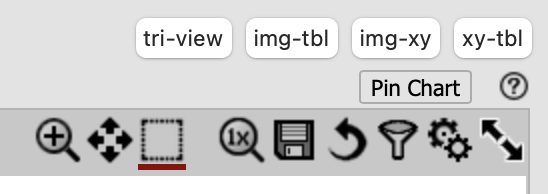
\includegraphics[width=3.12500in]{jira_imgs/3174.png}

}
\hdashrule[0.5ex]{\textwidth}{1pt}{3mm}
  Expected Result \\
{\footnotesize
The image table should appear on the right, with the image (``Data
Product'') viewer and the coverage image in tabs on the left. ~Only
r-band images should be shown.

}
\hdashrule[0.5ex]{\textwidth}{1pt}{3mm}
  Actual Result \\
{\footnotesize

}
\begin{tabular}{p{2cm}p{14cm}}
\toprule
Step 7 & Step Execution Status: \textbf{ Not Executed } \\ \hline
\end{tabular}
 Description \\
{\footnotesize
Select the coverage image tab.

}
\hdashrule[0.5ex]{\textwidth}{1pt}{3mm}
  Expected Result \\
{\footnotesize
The coverage tab should display the frames of all the images returned
from the search.

}
\hdashrule[0.5ex]{\textwidth}{1pt}{3mm}
  Actual Result \\
{\footnotesize

}
\begin{tabular}{p{2cm}p{14cm}}
\toprule
Step 8 & Step Execution Status: \textbf{ Not Executed } \\ \hline
\end{tabular}
 Description \\
{\footnotesize
Use the layers dialog, from the ``Manipulate overlay display'' button in
the image toolbar:\\
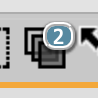
\includegraphics[width=0.37500in]{jira_imgs/3175.png}to change the
display of image frames from ``all'' to ``selected''. (This shows only
the frames of images that are selected using the checkbox in their table
row.)\\
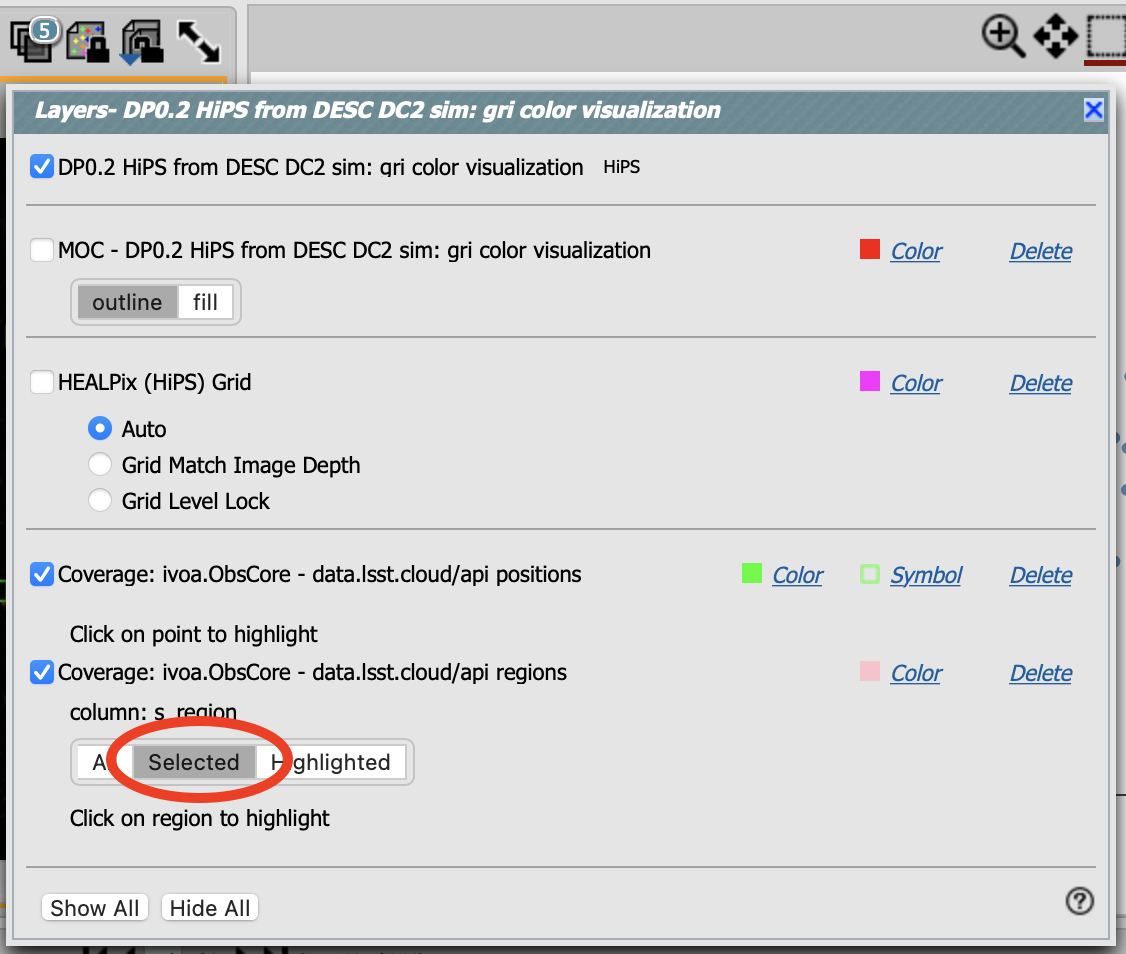
\includegraphics[width=3.12500in]{jira_imgs/3176.png}

}
\hdashrule[0.5ex]{\textwidth}{1pt}{3mm}
  Expected Result \\
{\footnotesize

}
\hdashrule[0.5ex]{\textwidth}{1pt}{3mm}
  Actual Result \\
{\footnotesize

}
\begin{tabular}{p{2cm}p{14cm}}
\toprule
Step 9 & Step Execution Status: \textbf{ Not Executed } \\ \hline
\end{tabular}
 Description \\
{\footnotesize
Click on the header of the ``t\_min'' column to sort the data in
increasing order of time.

}
\hdashrule[0.5ex]{\textwidth}{1pt}{3mm}
  Expected Result \\
{\footnotesize
Two coadded images, one ``deep'' (dataproduct\_subtype =
lsst.deepCoadd\_calexp) and one ``good seeing'' (lsst.goodSeeingCoadd),
of the same sky tile, should appear at the top of the list (NB: coadded
images do not have times assigned in the DP0.2 dataset; this will be
changed in later data releases).

}
\hdashrule[0.5ex]{\textwidth}{1pt}{3mm}
  Actual Result \\
{\footnotesize

}
\begin{tabular}{p{2cm}p{14cm}}
\toprule
Step 10 & Step Execution Status: \textbf{ Not Executed } \\ \hline
\end{tabular}
 Description \\
{\footnotesize
Use the checkboxes to select the two coadded images at the top of the
list.\\
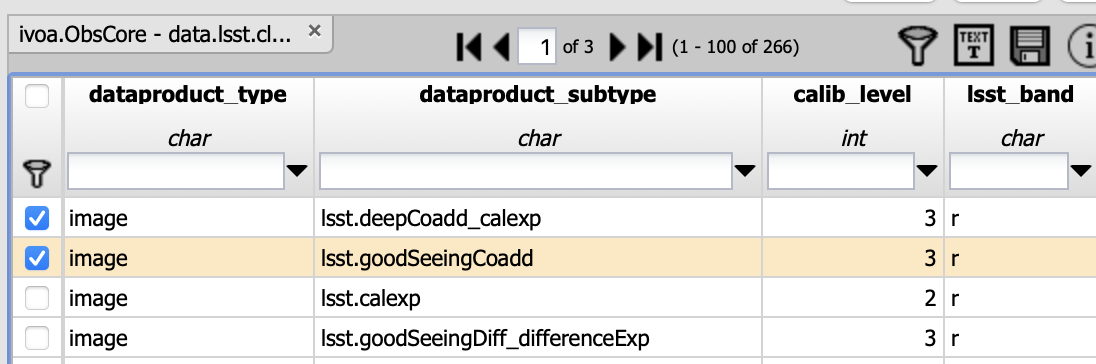
\includegraphics[width=3.12500in]{jira_imgs/3177.png}

}
\hdashrule[0.5ex]{\textwidth}{1pt}{3mm}
  Expected Result \\
{\footnotesize
Their (identical) frames should appear in the coverage image.

}
\hdashrule[0.5ex]{\textwidth}{1pt}{3mm}
  Actual Result \\
{\footnotesize

}
\begin{tabular}{p{2cm}p{14cm}}
\toprule
Step 11 & Step Execution Status: \textbf{ Not Executed } \\ \hline
\end{tabular}
 Description \\
{\footnotesize
Look down in the list to the two single-epoch CCD images (a coadd and a
difference image) from visit 193110 (see the ``lsst\_visit'' column).
~These should be the 7th and 8th in the table. ~Use the checkboxes to
select these.\\[2\baselineskip](This visit is chosen for this test case
because it's at a distinctive angle to the coadd
tiles.)\\[2\baselineskip]Zoom the coverage display so that it clearly
displays the frames of both the coadds and the single-epoch images.

}
\hdashrule[0.5ex]{\textwidth}{1pt}{3mm}
  Expected Result \\
{\footnotesize
There should now be four images selected.

}
\hdashrule[0.5ex]{\textwidth}{1pt}{3mm}
  Actual Result \\
{\footnotesize

}
\begin{tabular}{p{2cm}p{14cm}}
\toprule
Step 12 & Step Execution Status: \textbf{ Not Executed } \\ \hline
\end{tabular}
 Description \\
{\footnotesize
Use the ``Filter on selected rows'' control in the table header\\
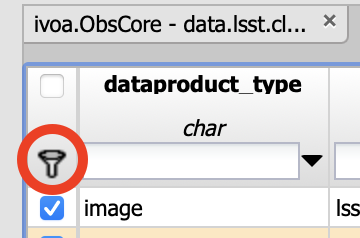
\includegraphics[width=1.69792in]{jira_imgs/3178.png}to limit the
display to only the selected images.

}
\hdashrule[0.5ex]{\textwidth}{1pt}{3mm}
  Expected Result \\
{\footnotesize
Only the four selected images should remain in the table.

}
\hdashrule[0.5ex]{\textwidth}{1pt}{3mm}
  Actual Result \\
{\footnotesize

}
\begin{tabular}{p{2cm}p{14cm}}
\toprule
Step 13 & Step Execution Status: \textbf{ Not Executed } \\ \hline
\end{tabular}
 Description \\
{\footnotesize
Select the ``Data Product'' tab. ~Use the ``Show full grid'' control in
the image toolbar\\
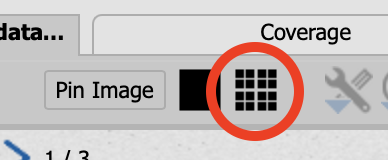
\includegraphics[width=3.12500in]{jira_imgs/3179.png}to show all four
images at once.

}
\hdashrule[0.5ex]{\textwidth}{1pt}{3mm}
  Expected Result \\
{\footnotesize
The images should be displayed in a 2x2 grid.\\[2\baselineskip]One image
will be highlighted with a yellow/orange border, following the
highlighted row in the table.\\[2\baselineskip](Note that the image
display itself does not clearly indicate which image is which; this is a
known deficiency and will be addressed by future changes to the back-end
image services and the Portal. ~In the mean time, the image metadata
table highlight can be used to explore which is which.)

}
\hdashrule[0.5ex]{\textwidth}{1pt}{3mm}
  Actual Result \\
{\footnotesize

}
\begin{tabular}{p{2cm}p{14cm}}
\toprule
Step 14 & Step Execution Status: \textbf{ Not Executed } \\ \hline
\end{tabular}
 Description \\
{\footnotesize
If the test started in a fresh session, the images will normally be
initially displayed each in its own natural row/column
orientation.\\[2\baselineskip]Highlight one of the coadded images in the
table. Then select the ``Align and lock by WCS'' control in the image
toolbar.\\
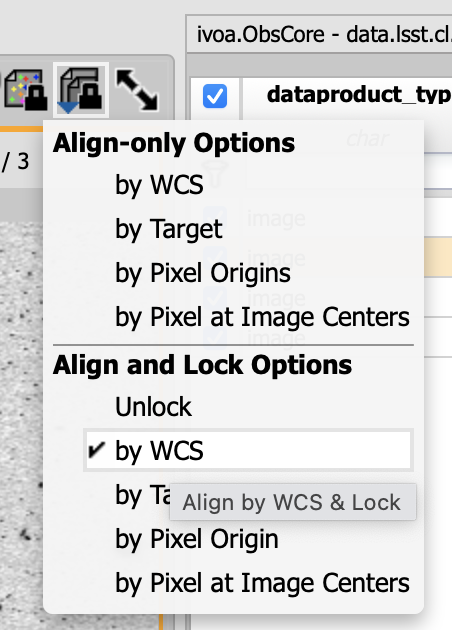
\includegraphics[width=2.07292in]{jira_imgs/3180.png}

}
\hdashrule[0.5ex]{\textwidth}{1pt}{3mm}
  Expected Result \\
{\footnotesize
All four images should now be displayed at the same orientation and
scale. ~Note that the Visit-193110 images appear significantly rotated.

}
\hdashrule[0.5ex]{\textwidth}{1pt}{3mm}
  Actual Result \\
{\footnotesize

}
\begin{tabular}{p{2cm}p{14cm}}
\toprule
Step 15 & Step Execution Status: \textbf{ Not Executed } \\ \hline
\end{tabular}
 Description \\
{\footnotesize
Zoom and pan on the images to verify that they move
together.\\[2\baselineskip]Enjoy the comparison of the single-epoch and
coadded image depths, and the comparison of the single-epoch image and
the difference image. (Note: in the DP0.2 production, the ``good
seeing'' coadd was used as the template image for the image
differencing.)

}
\hdashrule[0.5ex]{\textwidth}{1pt}{3mm}
  Expected Result \\
{\footnotesize

}
\hdashrule[0.5ex]{\textwidth}{1pt}{3mm}
  Actual Result \\
{\footnotesize

}




% This appendix is put in as part of the template. You may edit and add to it.
% It is not overwritten by Docsteady.

\newpage
\appendix
\section{Documentation}
The verification process is defined in \citeds{LSE-160}.
The use of Docsteady to format Jira information in various test and planing documents is
described in \citeds{DMTN-140} and practical commands are given in \citeds{DMTN-178}.

\section{Acronyms used in this document}\label{sec:acronyms}
\input{acronyms.tex}

\newpage

% Uncomment this if Docsteady makes you additional appendix
%\input{DMTR-381.appendix.tex}

\end{document}
